\documentclass[12pt,a4paper]{article}
\usepackage[utf8x]{inputenc}
\usepackage[pdftex]{graphicx}
\PrerenderUnicode{äöüÄÖÜß}
\usepackage[ngerman]{babel}
\usepackage{enumitem}
\usepackage{amsmath}
\usepackage{color}
\usepackage[paper=a4paper,left=15mm,right=15mm,top=35mm,bottom=25mm]{geometry}
\usepackage{enumitem}
\setitemize{noitemsep}

\usepackage{titling}
\setlength{\droptitle}{-4cm}

\title{Ausarbeitung WebTech II}
\author{N. Henczi, B. Kleinhückelkoten, D. Kühn, D. Mues, D. Wirkner}
\date{30.4.2013}
\begin{document}	
\maketitle
\thispagestyle{empty}
\pagestyle{empty}

\newcommand{\TODO}[1]{\colorbox{red}{TODO: #1}}
	
\section{Einführende Phase}
In der Planung des Projekts wurden hauptsächlich drei Aspekte der Applikation diskutiert. Dies waren zunächst die \textbf{Technologien} welche die Arbeit in der Gruppe vereinfachen sollten, dann die \textbf{technischen Aspekte} und Entscheidungen, wie das Backend umgesetzt werden sollte und mit der deutlich meisten Euphorie \textbf{Aufbau und Aussehen} des Projekts.

\subsection{Eingesetzte Technologien}
Wir entschieden uns, in unserem Projekt die in der Vorlesung vorgestellten Technologien zu benutzen. Dies beinhaltet:

\begin{itemize}
\item \textit{Maven} als Buildprogramm, da es sehr einfach zu nutzen ist und gleichzeitig übersichtlich und komfortabel nutzbar ist
\item \textit{Jetty} als Server, da er mit Maven bereits mitgeliefert ist und in seinem Umfang unseren Ansprüchen vollkommen genügt
\item \textit{Hibernate} als Datenbank Schnittstelle, \TODO{warum haben wir Hibernate genommen?}
\end{itemize}

Die Kommunikation wurde dadurch, dass wir uns ein- bis zweimal jede Woche trafen auf Mailverkehr beschränkt. Das genügte, da wir von vornherein planten dass jeder seinen Aufgabenbereich kennen sollte und am Schluss die verbleibenden Aufgaben frühzeitig verteilt werden sollten. So hatten wir die Möglichkeit, alle Mitglieder zu erreichen um im Vorfeld Dinge oder Probleme anzusprechen und konnten diese dann auf den Treffen klären. \\

Um die Koordination in der Gruppe zu ermöglichen benutzten wir zusätzlich ein Versionskontrollsystem. Wir entschieden uns für \textit{GIT}, da es hier über GitHub (www.github.com) sehr einfach möglich war ein Repository anzulegen.

Da nur zwei Mitglieder mit GIT vertraut waren und auch nicht alle die Vorlesung in der Maven behandelt wurde besucht hatten, nutzte unsere Gruppe ein paar der ersten Termine zum Kennenlernen und Erklären von GIT und Maven.

\subsection{Entscheidungen in der Implementierung}
Bevor wir uns der Implementierung widmen konnten empfanden wir es als nützlich die Terminologie zu klären. Es war gemeinsamer Konsens, dass wir User haben würden, die Shouts verfassen.

Ein User $U_A$, der einem User $U_B$ ermöglichen möchte seine Nachrichten $M_{A0} \dotsc M_{An}$ einzusehen, kann $U_B$ einen \textbf{Invite} schicken. Nimmt $U_B$ diese Einladung an, ist $U_B$ ein \textbf{Fan} von $U_A$, gleichzeitig ist $U_A$ ein \textbf{Idol} von $U_B$. \\

Wir waren uns einig, dass es für unser Projekt nur diese zwei Model-Classes geben würde, \verb+Message+ (statt Shout, da Message technischer und weniger speziell ist) und \verb+User+. Welche Attribute diese Klassen haben sollten, wurde allerdings von unserer anfänglichen Idee nochmal leicht abgewandelt. 

Unser Plan war zu Beginn, dass ein User nur zwei Listen von Usern haben sollte, nämlich die Idols und die, die einen Invite geschickt bekamen. Die Logik hätte dann einen Umweg über den jeweils anderen User und dessen Idol-Liste machen müssen, was aber doppeltes Eintragen von User-Relationen verhindert hätte.

Durch das Konzept der inversen Abhängigkeit \TODO{ist es die inverse Abhängigkeit?} kann man diesen Vorteil aber beibehalten und dennoch den Komfort ermöglichen, bidirektional auf die Idols und Fans zugreifen zu können.

\subsection{Aufbau und Aussehen}
Damit wir mit dem Projekt beginnen konnten, mussten wir natürlich zu Beginn festlegen, wie es aussehen sollte. Dazu gehörte zunächst der Aufbau der Applikation, also die Unterteilung in Pages und Components. Zu den letztendlichen Entscheidungen, wie und warum wir die jetzt eingesetzte Variante gewählt haben, siehe \TODO{section von Nico}.

Wir gingen diese Aufgabe an, indem wir mit Inkscape ein SVG erstellten, das abstrakt den Aufbau der verschiedenen Seiten darstellte. Da diese abstrakten Darstellungen auch im SVG File aus gruppierten Komponenten bestanden, konnten wir diese sehr leicht verschieben, verändern und von unserem zunächst vorgestellten Modell auf eine Lösung mit sehr viel weniger redundanten Pages und vielen gemeinsam nutzbaren Components kommen.

\begin{figure}[h!]
\begin{center}
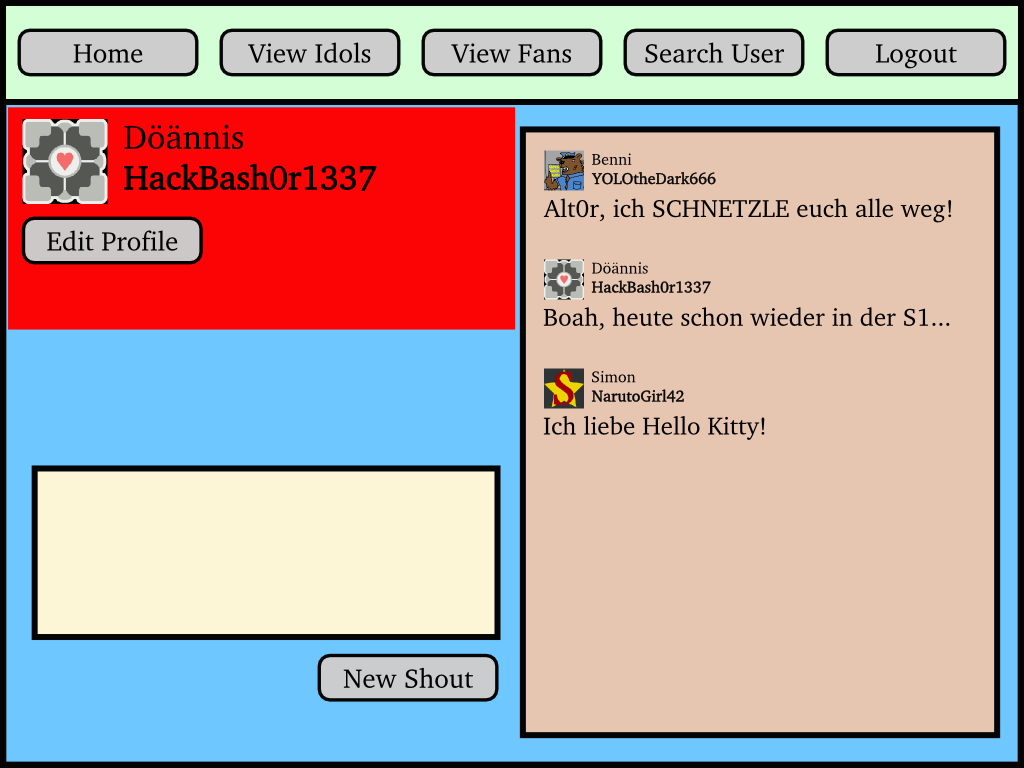
\includegraphics[width=0.9\textwidth]{entwurf.png}
\caption{Die erste Version der Ansicht zum betrachten des eigenen Profils}
\end{center}
\end{figure}


\subsection{Besondere Features und Name des Projekts}
Um das Projekt über die grundlegenen Anforderungen hinaus zu erweitern, haben wir einige Ideen für Features gesammelt, die mit realisiert werden könnten um ShoutCrowd -- wie unser Projekt genannt wurde -- noch cooler zu machen.

Der Name ShoutCrowd kam im Umfeld eines Metal-basierten Themes zustande. Eine unserer ersten Ideen war es, viele verschiedene Themes anzubieten, die der User selbst auch um eigene Themes hätte erweitern können. So wären die \verb+.properties+-Files für jedes Theme unterschiedlich und der ``Verfasse Nachricht''-Button könnte im Metal Theme ``Shout something awesome'' betitelt sein, im Gentlemen Society Theme ``Tell your fine chaps'' oder im Pirate Theme ``Name yer demand!''. An manchen Stellen wurden die besten dieser Ideen in das letztendliche Design der Seite übernommen. \\

Zudem wirkte die Seite in unseren vorgefertigten Skizzen ein wenig leer, wenn nur die Nachrichtentexte und die Namen der Verfasser angezeigt worden wären. Darum gaben wir jedem User noch die Möglichkeit, einen Avatar hochzuladen und einen persönlichen, änderbaren Nickname einzutragen. Das minutengenaue Datum der Nachricht wird ebenfalls mit angezeigt.

\newpage
\section{Layout}
\subsection{Einleitung}
Das Layout eines Webprojektes ist das erste, was dem Benutzer bei Benutzung eines solchen auffällt. Bei der Planung des Layouts wurde darum auf mehrere Aspekte eingegangen. Es soll schnell laden, übersichtlich, einfach zu bedienen und zentral veränderbar sein während es
optisch ansprechend sein soll. In den folgenden Abschnitten geht es um die Lösungsansätze, die wir zu den obigen Herausforderungen gewählt haben.

\subsection{Veränderbarkeit}
In dem Modul Webtechnologien 1 wurden im Zusammenhang mit veränderlichem Layout, die Cascading Style Sheets (css) propagiert, so dass sie für uns erste Wahl waren. Es wurden, unabhängig von den dynamischen Inhalten, HTML-Dateien angelegt, die aus <div> - Elemente und darin enthaltenen statischen Text (Platzhalter für dynamische Inhalte) bestehen. Diesen <div>s wurden Klassen und Ids zugewiesen, welche dann zentral von einer layout.css ihr optisches Erscheinungsbild bekommen haben. Die CSS konnte auf Grund der Projektgröße noch per Hand erstellt werden. Auf die Verwendung von Inline-definierten Styles wurde größtenteils verzichtet, da dadurch die Möglichkeit einer zentralen Veränderung des Styles abhanden kommen würde. 
Aus den gut kommentierten HTML-Dateien konnte dann jeder Ersteller einer Komponente/Page den, für ihn relevanten Teil extrahieren und daraus seine projektbezogene TML erzeugen. Verwendet wird eine klassische Aufteilung der div-Elemente. So gibt einen Header und einen Fotter. Dazwischen ist der 
$_{content}$"-
div zu finden, der auf Profilseiten, links Platz für die 
die Profilinformationen und rechts Platz für $_{Shouts}$"
(croaks) hat und auf allen andern Seiten Platz für entweder eine Auflistung, ein Formular, oder einen Text bietet. Positive Nebeneffekte der erzeugten HTML waren, dass klar definiert war, wie das Projekt mal aussehen würde und dass Dinge deutlich wurden, die bei der ursprünglichen Planung vergessen und/oder weniger gut durchdacht worden sind.
  
\begin{figure}[h!]
\begin{center}
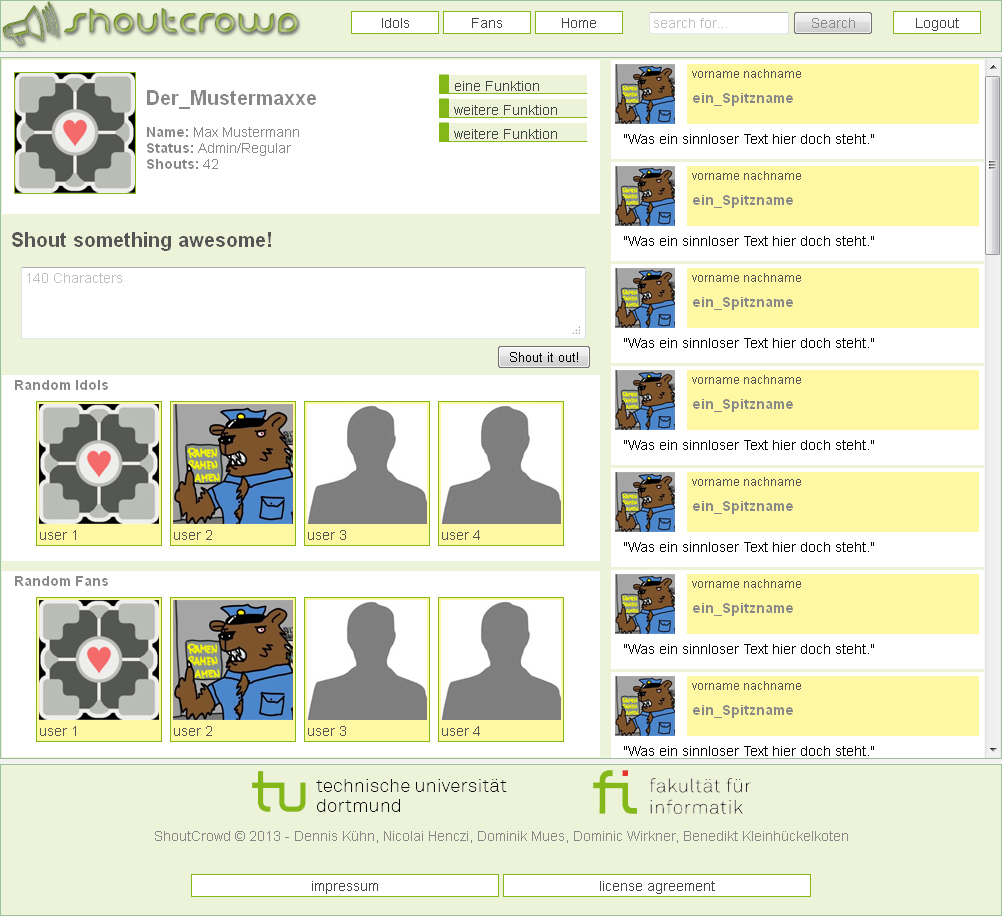
\includegraphics[width=0.9\textwidth]{first.jpg}
\caption{erstes Layout -- HTML mit statischen Inhalten per css optisch angepasst}
\end{center}
\end{figure}

\subsection{Ladezeit}
Lange Wartezeiten zwischen einem Request und der Response resultieren oft daher, dass viele größere Bilder geladen werden müssen. Um das möglichst zu verhindern sind nur wenige Grafiken mit einer begrenzten Farbpalette (reduziert Dateigröße) in das Grundlayout eingeflossen. Enthalten sind ein eigenes Logo und die Logos der Universität und der Informatikfakultät, so wie ein Bild einer jubelnden Menge, welches zur Begrüßung angezeigt wird.

\subsection{Haptik}
Die Wahrnehmung spielt nicht nur bei größeren Webprojekten mit vielen Funktionen eine große Rolle. Schon bei dem, doch recht beschaulichen, Projekt eines Twitter-Clons fallen viele Funktionen an, die Kontextspezifisch angeordnet werden müssen. So macht etwa ein "Profil bearbeiten"-Funktionen in einem Such Kontext keinen Sinn. Unsere Aufteilung beinhaltet eine Kopfnavigation mit den meistgenutzten Links (Idols, Fans, Home) und dem Logout-Button, so wie der Suche. Diese Seiten sollen von jedem Kotext aus erreichbar sein*. Derart nebeneinander aufgelistete Funktionen in der Kopfzeile sind im Web 2.0 häufig zu finden und sollten desshalb vielen Nutzern bekannt vorkommen und einen intuitiveren Umgang mit der Seite ermöglichen. Deutlich seltener genutzt werden Impressum, oder Lizenzvereinbarung. Diese Menüpunkte sind desshalb im Footer anzutreffen (welcher auch auf jeder Seite angezeigt wird). Kontextsensitiv sind Funktionen, wie beispielsweise "Invite Fan" oder "Edit Profile". Derartige Aufrufe sind nur möglich in einer
 Auflistung von Usern (z.B. über die Suche) oder direkt auf der Profilseite dieses Benutzers. Idealerweise wäre der "Edit Profile"-Menüpunkt ein Unterpunkt von dem typischweise in der Kopfzeile befindlichen "Settings"-Menüpunkt  gewesen. Da wir jedoch, zeitlich bedingt, auf die Implementierung weiterer Benutzereinstellungen verzichtet haben und die Kopfzeile sonst überladen wirken würde, wurde dieser Aspekt verworfen. Ebenfalls der Übersichtlichkeit und Gewohnheit der Benutzers geschuldet ist die Tatsache, dass jeder login/username nur in Verbindung mit seinem Avatar erscheint. Für den Fall, dass viele "Shouts" aufgelistet werden müssen, ist, um ein endloses Scrollen durch die Beiträge zu verhindern, eine Verteilung der Nachrichten auf mehrere Seiten implementiert (Pagination).  
*außer man ist nicht angemeldet; dann ist der logout-Button ein login-Button und die anderen Links führen auf die Startseite.

\subsection{Optische Wahrnehmung}
Die Optik in unserem Projekt war etwas, dass das wir ursprünglich vorhatten, zum Ende hin zu optimieren. Wie sich aber herrausstellt, ist das anfänglich gewählte Layout durchaus mehr als ausreichend für den Projektumfang. Farblich wurde der Stil auf weiß für den Hintergrund, pastell gelblich bzw. grünlich für Rahmen, <div>-Hintergrundfarben und Links, schwarz für Schrift und rot für Fehlermeldungen und wichtige Hinweise festgesetzt. Durch die Rahmen, die die einzelnen Komponenten( in den div-Elementen enthalten) voneinander trennen, wirkt die Seite aufgeräumter und bekommt eine klarer definierte Struktur. Abweichend von der ursprünglich gewählten Ansicht, wird der Benutzer auf der Startseite von einem Bild einer jubelnden Menge "begrüßt" welches farblich und thematisch zum Rest des Projektes passt. Das Erscheinungsbild des Projektes wäre ausbaufähig zu einem kompletten Corporate Design.

\subsection{Aufteilung der Komponenten/Pages}
Die Gestaltung und Verteilung der <div>s hat indirekte und direkte Auswirkungen auf Struktur der Komponenten und Pages. Nachdem es ein dreigliedriges Layout sein soll(Header, Content, Footer), macht es Sinn eine Komponente zu realisieren, die eben dieses Layout umsetzt. Innerhalb dieser Komponente wird die fest plazierte Komponente UserMenu (Header) und der Footer (nicht als Komponente, da der Inhalt des Footers nicht dynamisch ist), so wie eine body-Komponente, deren Inhalt von der aufrufenden Page bestimmt wird, angezeigt. Damit die Pages nicht zu unübersichtlich groß werden, sind einige Teile in Komponenten ausgelagert. Folgende Pages und Komponenten sind im Projekt enthalten:

\subsubsection{Pages}
1.CreateAccount: Implementierung einer Benutzer Registrierung
2.EditProfile: Formular zum bearbeiten der angegebenen Benutzerdaten
3.Home: eigene Profilseite mit Profilinformationen und Shouts
4.Imprint: Obligatorisches Impressum (Platzhalter)
5.Index: Startseite, die zum Login oder zur Registrierung aufruft
6.Licence: Lizenzvereinbarung (nur Platzhalter für Rechtskräftigen Content) 
7.Login: Formular zum einloggen
8.Test: Testseite für die Entwickler (nicht für den normalen Benutzer gedacht)
9.ViewList: Auflistung von Usern durch Suche, Fans oder Idols
10.ViewProfile: wie Home, jedoch für fremde Profile
11.WipeAllData: Reset (für Angluin)

\subsubsection{Komponenten}
1.CreateMessage: Formular zur Eingabe von Shouts
2.Layout: (Erklärung siehe oben)
3.Pagination: Seitenzähler für Shouts
4.ProfileActions: Kontextabhängige Funktionsbuttons (Links)
5.ProfileDetails: selbererklärend
6.ProfileListItem: Ansicht eines einzelnen Users in einer Auflistung
7.SingleMessage: Ansicht eines einzelnen Shouts
8.UserMenu: Die Kopfzeilen Navigation

\subsection{Abschließendes und Probleme}
Ziele unserer Gestaltung des Layouts sind eine einfache Umsetzung, ein komponentenunabhängiges Erscheinungsbild (zusammenpassend) und eine intuitive und leichte Bedienbarkeit. Zu letzterem ist zu sagen, dass für das Erreichen jeder Seite maximal drei Klicks notwendig sind und dem Benutzer entgegen gekommen wird, falls er beim Ausfüllen der Formulare etwas falsch gemacht hat. Komponentenunabhängigkeit ist durch eine nicht vorhandene statische Breitenzuweisung ebenfalls gewährleistet, was jedoch den Entwicklern die Möglichkeit bieten würde, Komponenten zu erstellen, die das Layout zerreißen würden. Dieses Problem ließe sich nur durch individuell angepasste Styles für jede Komponente verhindern. Die Umsetzung des Layouts und die spätere Einbindung in das Tapestry Projekt, erwies sich, bis auf kleinere Schwierigkeiten bei den Browserabhängigkeiten, als vergleichsweise einfach. Tapestry bietet allerdings keine (uns bekannte) Möglichkeit in CSS-Datein, Relative Pfade zu verwenden, wie dies in den TMLs möglich ist (Bsp:  \verb+<img src="${UserImage}" alt="pic"/>+ ). Ausgehend von von den genannten Zielen und durchdachten Aspekten ist zu sagen, dass vieles mit einfachen Mitteln realisiert und dennoch nicht unterspezifiziert ist. 

\newpage
\section{Schlussbemerkungen}

\subsection{Ausblick}
Eine Webapplikation ist nie ganz fertig. Da die Zeit für unser Projekt jedoch begrenzt ist und die Shoutcrowd nie wirklich online gehen wird noch ein paar Worte, um zu zeigen in welche Richtung man das Projekt ausweiten könnte. Zunächst ein paar Funktionen, die in der Realität anders gelöst werden müssen:
Ein Reset der Applikation müsste normalerweise durch einen Administrator geschehen. Für einen Administrator benötigt man jedoch ein Rechtesystem und eine Extra Administratorseite. Da dies  für die reine Funktionalität nicht relevant ist haben wir es nicht implementiert. Für die Selenium Test's wird jedoch ein solcher Reset der Datenbank benutzt um durch den Angluin Algorithmus den Applikations-Graph zu lernen. Deshalb haben wir unter der URL (http://localhost:8080/shoutcrowd/wipealldata)
Eine Seite erstellt, die bei Eingabe des Richtigen Resetcode (doreset), einen Reset der Datenbank veranlasst. Des weiteren würden in der Realität Passwörter nicht im Klartext in der Datenbank gespeichert. Auch hier wurde der Einfachheit halber auf entsprechende Verschlüsselung verzichtet.

Unsere gesamte Applikation ist recht statisch es gibt kein Dynamisches Nachladen von Inhalten. Somit bekommt es der eingeloggte User nicht mit, wenn einer seiner Idols etwas neues "shouted", es sei denn er lädt die Seite neu. Deswegen wäre für die Zukunft ein Automatisches Neuladen der Nachrichten in kleinen Zeitabständen ein nettes feature. Bei der suche könnte auch bereits beim eintippen eine Liste mit passenden Ergebnissen geladen werden aus der man bereits auswählen kann. 
Gut wäre außerdem eine Zuordnung von Usern auf verschiedene "crowd's" Man könnte dann die "shouts" nach "crowd's" sortiert anzeigen lassen und hätte so eine bessere Übersicht, gerade bei vielen Idols.
Zu guter Letzt wäre auch ein Recommender System denkbar, da unter dem Eingabefeld für die Messages noch so viel freier Platz ist könnte man diesen mit Profilbildern von anderen Usern füllen. Hier könnten Personen mit den gleichen Idols oder Personen deren Fans eigene Idols sind angezeigt werden. So wäre es einfacher neue Idols zu finden und unsere Applikation würde Sozialer.

\subsection{Fazit}
Die Shoutcrowd läuft ohne Fehler und man kann Problemlos User anlegen, Messages schreiben und andere User einladen einem selbst zu folgen. Doch bis da hin war einiges zu tun.
Die Gruppe hatte sich schnell gefunden, die meisten saßen in der ersten Vorlesung nebeneinander.
Die einzelnen Gruppenmitglieder waren von ihren Vorkenntnissen sehr inhomogen, so gab es Personen mit viel Vorwissen, die bereits eigene Webanwendungen gebaut hatten und andere die noch nie die Wörter Tapestry, Maven oder Selenium gehört und sich mit Webentwicklung auseinander gesetzt hatten.
Wir einigten uns schnell darauf das Versionskontrollsystem GitHub zu benutzen um so alle gut am Projekt arbeiten zu können. Diese Entscheidung war rückblickend eine sehr gute, denn ein Versionskontrollsystem ist bei einer Gruppenarbeit dieser Art fast unentbehrlich und hat vieles vereinfacht.
Zuerst wurde der Grobe Aufbau und die verschiedenen Ansichten skizziert und überlegt was man zur Umsetzung benötigt. Wir verfolgten den Ansatz eines "Rock-Theme" und dadurch entstand dann der Name: Shoutcrowd. Wir überlegten uns Im Rahmen dieses Theme, dass User die mir Folgen Fans heißen sollen und das User denen ich folge Idols genannt werden könnten. Außerdem waren wir gegen Freundeslisten und Freunde, da wir dies bei den beiden Listen für Fans und Idols nicht mehr für sinnvoll hielten. Die vielen Besprechungen am Anfang sorgten dafür das jedes Gruppenmitglied die gleiche Vorstellung bekam wie das Projekt grob aufgebaut werden sollte.
Dann legten wir ein Projekt und eine Erste Klassenstruktur an und verteilten Aufgabenbereiche. So entstand Shoutcrowd so wie es jetzt ist. Wir trafen uns über das Semester hinweg regelmäßig um anderen Mitgliedern Zuhause erstellten Code zu erläutern oder Erkenntnisse weiterzugeben und zu helfen wo Probleme auftauchten. In Emails und einer Textdatei im Repository wurden Aufgaben, die noch zu bearbeiten waren festgehalten, damit man ihre Bearbeitung nicht vergaß. Dieses Vorgehen war, da nicht immer alle zu den treffen erscheinen konnte sehr hilfreich.
Die Zeit wurde zum Ende des Projekts etwas knapp, was aber für diese Art von Projekten normal zu sein scheint, zumal immer noch etwas verbessert werden kann.
Die Tatsache, dass alles was in der Shoutcrowd geschrieben wird von jedem User gelesen werden kann, wenn dieser nur auf das entsprechende Profil geht macht unsere Seite freier und offener für die User, die nicht viele Freunde haben oder neue Leute kennen lernen möchten. So kann jeder bei jedem lesen und benötigt keine Freundschaft mit dem entsprechenden User. Wenn ein User Interessante Nachrichten schreibt sieht man das und kann diesem daraufhin folgen. Die Entscheidung gegen Freundeslisten hat also viele Vorteile auch wenn uns die Verschiedenen Fan und Idol Listen anfangs etwas verwirrten.
Insgesamt verlief die Zusammenarbeit gut und gerade den Mitgliedern des Teams, die über wenig Vorkenntnisse verfügten konnte bei den vielen treffen vieles noch einmal erklärt werden, sodass das Projekt bei alles Mitgliedern des Teams viel an Erfahrung im Umgang mit den in der Vorlesung vorgestellten Technologien gebracht hat.
\end{document}